%% =============================================================
%%  Les accords — de l'accord parfait à la septième diminuée
%%  Guide de référence, composé en LaTeX, gravures LilyPond
%% =============================================================
%%
%%  Les figures (gravures/a-*.cropped.pdf), les tableaux et les
%%  réponses de l'exercice (gravures/accords-*.tex) et le fichier
%%  accords.musicxml sont produits par outils/generer_accords.py, à
%%  partir du modèle de hauteurs des autres guides (outils/gammes.py,
%%  outils/intervalles.py). Voir le colophon en dernière page.
%%
\documentclass[a4paper,11pt]{article}

\usepackage[top=2.2cm,bottom=2.4cm,left=2.2cm,right=2.2cm]{geometry}
\usepackage[T1]{fontenc}
\usepackage[utf8]{inputenc}
\usepackage[french]{babel}
\usepackage{lmodern}
\usepackage{amsmath}
\usepackage{xcolor}
\usepackage{graphicx}
\usepackage{titlesec}
\usepackage{fancyhdr}
\usepackage{mdframed}
\usepackage{enumitem}
\usepackage{booktabs}
\usepackage{hyperref}

\graphicspath{{gravures/}}

% ---- Couleurs, reprises du document des accords de guitare ---------
\definecolor{navy}{RGB}{18,50,105}
\definecolor{lightnavy}{RGB}{235,241,255}
\definecolor{mygray}{RGB}{110,110,110}

\hypersetup{colorlinks=true, linkcolor=navy, urlcolor=navy,
  pdftitle={Les accords — de l'accord parfait à la septième diminuée},
  pdfauthor={Fabian Bastin}}

% ---- En-tête et pied -----------------------------------------------
\pagestyle{fancy}
\fancyhf{}
\renewcommand{\headrulewidth}{0.4pt}
\renewcommand{\footrulewidth}{0.4pt}
\fancyhead[L]{\small\bfseries\textcolor{navy}{Les accords}}
\fancyhead[R]{\small\textcolor{mygray}{\thepage}}
\fancyfoot[C]{\small\textcolor{mygray}{De l'accord parfait à la septième diminuée}}

% ---- Titres de section ---------------------------------------------
\newcommand{\navysect}[1]{%
  \colorbox{navy}{%
    \parbox[c][17pt]{\dimexpr\linewidth-2\fboxsep\relax}{%
      \color{white}\hspace{6pt}\bfseries\normalsize #1}}%
}
\titleformat{\section}[block]{\normalfont}{}{0pt}{\navysect}
\titlespacing*{\section}{0pt}{16pt}{10pt}

% ---- Encadré de remarque -------------------------------------------
\newmdenv[linecolor=navy, linewidth=0.5pt, backgroundcolor=lightnavy,
  innertopmargin=6pt, innerbottommargin=6pt,
  innerleftmargin=8pt, innerrightmargin=8pt,
  skipabove=8pt, skipbelow=8pt, nobreak=true]{remarque}

% ---- Chiffrages ------------------------------------------------------
% Un chiffre romain et ses chiffres empilés : \ch{V}{6}{5} donne V 6 sur 5.
\newcommand{\ch}[3]{\ensuremath{\mathrm{#1}^{#2}_{#3}}}
% Des chiffres seuls, empilés : \fig{6\\4}.
\newcommand{\fig}[1]{{\footnotesize\renewcommand{\arraystretch}{0.75}%
  \begin{tabular}[c]{@{}c@{}}#1\end{tabular}}}

% ---- Figure gravée ---------------------------------------------------
% Figure gravée, avec sa légende. Toutes les gravures sont à la même
% échelle, celle des gravures des mordants : leurs portées ont la même
% taille, quelle que soit leur largeur. Le tout tient dans une minipage :
% figure et légende ne sont jamais séparées par un saut de page.
\newcommand{\echelle}{1.16}
\newcommand{\gravure}[2]{%
  \par\medskip\noindent
  \begin{minipage}{\linewidth}
    \centering
    \includegraphics[scale=\echelle]{#1.cropped.pdf}\\[4pt]
    {\small\itshape\color{mygray} #2}
  \end{minipage}\par\medskip
}

\setlist{itemsep=2pt, topsep=4pt, parsep=0pt}

\begin{document}

% =====================================================================
\begin{titlepage}
\centering
\vspace*{3cm}
{\Huge\bfseries\color{navy} Les accords\par}
\vspace{0.6cm}
{\LARGE\color{navy} De l'accord parfait à la septième diminuée\par}
\vspace{1.4cm}
{\large Des tierces superposées, une basse qui décide\par}
\vspace{2.5cm}
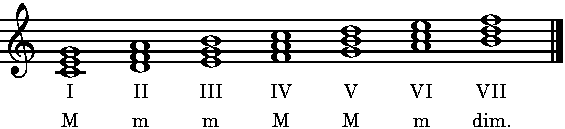
\includegraphics[scale=1.4]{a-degres-majeur.cropped.pdf}
\vfill
{\small\color{mygray}
Gravures LilyPond, composition \LaTeX.\\
Fichier MusicXML joint.\par}
\vspace{1cm}
\end{titlepage}

\tableofcontents
\newpage

% =====================================================================
\section{Avant-propos}

Un \textbf{accord} est la rencontre d'au moins trois sons de noms différents,
entendus ensemble. Dans la musique tonale, il se bâtit en superposant des
tierces. Au programme de matières théoriques de l'École de musique
Vincent-d'Indy, ces notions relèvent des niveaux 5 et 6 ; l'enchaînement des
accords --- cadences (\href{https://www.slashbin.net/musique/theorie/cadences.pdf}{\emph{Les cadences}}), écriture à quatre voix --- relève de
l'harmonie, qui
vient ensuite.

À lire après
\href{https://www.slashbin.net/musique/theorie/intervalles.pdf}{\emph{Les
intervalles}}, dont les tierces, les quintes et les septièmes sont la matière
de tout accord, et
\href{https://www.slashbin.net/musique/theorie/gammes.pdf}{\emph{Les
gammes}}, qui nomment les degrés et construisent la gamme mineure harmonique.

\begin{remarque}
\textbf{Conventions.} Les notes sont nommées en français. Les exemples sont
écrits en clé de sol, sans armure : chaque altération est écrite devant sa
note ; un seul y ajoute une portée en clé de fa, pour la basse. Les
intervalles sont abrégés comme dans \emph{Les intervalles} : 3ce~M pour une
tierce majeure, 3ce~m pour une tierce mineure, 5te~J pour une quinte juste,
dim. et aug. pour diminuée et augmentée.
\end{remarque}

Le fichier MusicXML joint fait entendre chaque exemple ; la
section~\ref{sec:musicxml} le présente.

% =====================================================================
\section{Des tierces superposées}
\label{sec:tierces}

\textbf{Une lettre sur deux.} Un accord se bâtit à partir d'une note, sa
\emph{fondamentale}, en empilant des tierces : sa \emph{tierce}, puis sa
\emph{quinte}, une tierce plus haut. Chaque note saute une lettre : sur sol,
on empile si, puis ré. Les noms des notes de l'accord sont ceux des
intervalles qu'elles forment avec la fondamentale.

\textbf{Trois ou quatre sons.} Fondamentale, tierce et quinte forment un
\emph{accord de trois sons}. Une tierce de plus apporte la \emph{septième} :
sol, si, ré, fa est un \emph{accord de quatre sons}.

\gravure{a-tierces}{Sol, puis sa tierce, sa quinte et sa septième : chaque
note prend une lettre sur deux.}

\textbf{Les noms restent attachés aux notes.} Disposées autrement, ou
doublées à l'octave, les notes gardent leur rôle : sol reste la fondamentale de
l'accord, même quand si est en dessous (section~\ref{sec:renversements}).

% =====================================================================
\section{Les quatre accords de trois sons}
\label{sec:natures}

Les deux tierces empilées sont chacune majeure ou mineure : quatre
combinaisons, quatre accords. On les distingue aussi par la tierce et la
quinte qu'ils forment au-dessus de leur fondamentale.

\gravure{a-natures}{Les quatre accords de trois sons, bâtis sur do.}

\begin{center}
%% Produit par outils/generer_accords.py — ne pas modifier à la main.
\begin{tabular}{@{}l l l l l@{}}
\toprule
\textbf{Accord} & \textbf{Tierce} & \textbf{Quinte} & \textbf{Tierces empilées} & \textbf{Sur do} \\
\midrule
parfait majeur & 3ce M & 5te J & 3ce M + 3ce m & do -- mi -- sol \\
parfait mineur & 3ce m & 5te J & 3ce m + 3ce M & do -- mi bémol -- sol \\
quinte diminuée & 3ce m & 5te dim. & 3ce m + 3ce m & do -- mi bémol -- sol bémol \\
quinte augmentée & 3ce M & 5te aug. & 3ce M + 3ce M & do -- mi -- sol dièse \\
\bottomrule
\end{tabular}

\end{center}

\textbf{L'accord parfait.} Il doit son nom à sa quinte juste. Majeur ou mineur,
il ne change que par sa tierce : une tierce majeure fait l'accord parfait
majeur, une tierce mineure l'accord parfait mineur. Leurs intervalles sont des
consonances : ce sont les accords du repos, ceux sur lesquels une pièce
s'achève. L'accord parfait majeur est même inscrit dans le son : les
harmoniques 4, 5 et 6 d'un do grave sont do, mi et sol
(\href{https://www.slashbin.net/musique/theorie/frequences.pdf}{\emph{Les
fréquences}}).

\textbf{Les quintes altérées.} L'accord de quinte diminuée empile deux
tierces mineures, l'accord de quinte augmentée deux tierces majeures. Leur
quinte est dissonante : ils sonnent instables et appellent une suite.

% =====================================================================
\section{Un accord sur chaque degré}
\label{sec:degres}

\textbf{Avec les notes de la gamme.} Sur chaque degré d'une gamme, on bâtit un
accord en ne prenant que des notes de cette gamme. On le désigne par le
chiffre romain de son degré : I sur la tonique, V sur la dominante.

\textbf{En majeur.} Les accords de I, IV et V sont des accords parfaits
majeurs, ceux de II, III et VI des accords parfaits mineurs ; VII porte un
accord de quinte diminuée. Ce schéma est le même dans les quinze tonalités
majeures : il ne dépend que de la place des tons et des demi-tons dans la
gamme.

\gravure{a-degres-majeur}{Un accord sur chaque degré de do majeur, sa nature
sous son chiffre romain : M pour un accord parfait majeur, m pour un mineur,
dim. pour un accord de quinte diminuée.}

\textbf{En mineur.} Les accords se bâtissent sur la gamme mineure harmonique,
celle qui a une sensible. C'est elle qui rend majeur l'accord de V : mi, sol
dièse, si en la mineur. Le même sol dièse fait de III un accord de quinte
augmentée.

\gravure{a-degres-mineur}{Un accord sur chaque degré de la mineur harmonique ;
aug. désigne l'accord de quinte augmentée.}

\textbf{Les trois accords principaux.} À eux trois, les accords de I, IV et V
emploient les sept notes de la gamme, en majeur comme en mineur harmonique :
chaque note de la gamme appartient à l'un d'eux au moins. Harmoniser une
mélodie simple commence par là.

\begin{remarque}
\textbf{Capitales ou minuscules.} Les chiffres romains s'écrivent ici tous en
capitales, comme dans la tradition française : le chiffre dit le degré, non
la nature de l'accord. L'usage anglo-saxon écrit en minuscules les accords
mineurs et de quinte diminuée --- ii, iii, vi, vii° en majeur.
\end{remarque}

% =====================================================================
\section{Position fondamentale et renversements}
\label{sec:renversements}

\textbf{La basse décide.} Un accord est en \emph{position fondamentale}
quand sa fondamentale est à la basse, la note la plus grave. Si c'est sa
tierce, il est au \emph{premier renversement} ; sa quinte, au \emph{deuxième
renversement}. Seule la basse compte : au-dessus d'elle, les autres notes
peuvent se disposer dans n'importe quel ordre et se doubler sans que la
position change.

\gravure{a-renversements}{L'accord de do majeur dans ses trois positions, et
leur chiffrage : la fondamentale, puis la tierce, puis la quinte à la basse.}

\textbf{Le chiffrage.} Il vient de la basse chiffrée de l'époque baroque, où
des chiffres posés sur la basse indiquaient à l'accompagnateur les intervalles
à jouer au-dessus d'elle. En position fondamentale, ce sont une tierce et une
quinte ; au premier renversement, une tierce et une sixte ; au deuxième, une
quarte et une sixte. La tierce va de soi et s'omet : le chiffrage se réduit à
5, 6 et \fig{6\\4}.

\begin{center}
%% Produit par outils/generer_accords.py — ne pas modifier à la main.
\begin{tabular}{@{}l l c c l@{}}
\toprule
\textbf{Position} & \textbf{À la basse} & \textbf{Complet} & \textbf{Abrégé} & \textbf{Sur do} \\
\midrule
position fondamentale & fondamentale & \fig{5\\3} & \fig{5} & do mi sol \\[7pt]
premier renversement & tierce & \fig{6\\3} & \fig{6} & mi sol do \\[7pt]
deuxième renversement & quinte & \fig{6\\4} & \fig{6\\4} & sol do mi \\[7pt]
\bottomrule
\end{tabular}

\end{center}

\textbf{Nommer un accord.} Hors de toute tonalité, on joint le chiffrage à la
nature : 5~M pour un accord parfait majeur en position fondamentale, 6~m pour
un accord parfait mineur au premier renversement, 6/4~M pour un accord parfait
majeur au deuxième. Dans une tonalité, le chiffre romain du degré vient
devant : \ch{I}{6}{}, \ch{IV}{6}{4}. En position fondamentale, le 5 s'omet :
on écrit I, IV, V.

\begin{remarque}
\textbf{Accord de sixte, accord de quarte et sixte.} La tradition française
nomme les renversements d'après leur chiffrage. Le deuxième est le moins
stable des trois : la quarte qu'il forme au-dessus de la basse passe pour une
dissonance dans l'harmonie classique (voir \emph{Les intervalles}), qui le
réserve à des emplois précis, comme l'accord de tonique en quarte et sixte
qui précède la dominante dans une cadence.
\end{remarque}

% =====================================================================
\section{La septième de dominante}
\label{sec:dominante}

\textbf{Sur le cinquième degré.} Une septième mineure ajoutée à l'accord
parfait majeur de la dominante donne la \emph{septième de dominante}, chiffrée
\ch{V}{7}{} : sol, si, ré, fa en do majeur. Mesurées depuis la fondamentale,
ses notes forment une 3ce~M, une 5te~J et une 7e~m.

\textbf{La même en majeur et en mineur.} En mineur, la sensible de la gamme
harmonique donne à la dominante le même accord : mi, sol dièse, si, ré, en la
majeur comme en la mineur. Parmi les accords de quatre sons qu'on bâtit sur
les degrés d'une gamme majeure ou mineure harmonique, c'est le seul de cette
structure, et il n'apparaît que sur V. Rencontrer une 3ce~M, une 5te~J et une
7e~m, c'est donc trouver la dominante ; la tonique est une quinte plus bas.

\textbf{Deux notes attirées.} L'accord réunit la sensible, si, et le quatrième
degré, fa, sa septième. Entre les deux, un triton : la quinte diminuée si--fa,
ou la quarte augmentée fa--si. C'est la tension de l'accord, et l'accord de
tonique la résout : la sensible monte d'un demi-ton vers la tonique, la
septième descend d'un degré vers la médiante --- d'un demi-ton en majeur,
d'un ton en mineur, où ré descend sur do en la mineur. La quinte diminuée
si--fa se resserre ainsi en tierce majeure, do--mi ; la quarte augmentée fa--si
s'ouvre en sixte mineure, mi--do.

\gravure{a-resolution}{La septième de dominante résolue sur l'accord de
tonique, en do majeur : si monte à do, fa descend à mi, sol reste en place, et
la basse va de la dominante à la tonique. La quinte, ré, est omise ; l'accord
de tonique est complet.}

\textbf{Ses renversements.} À quatre sons, quatre positions : la septième
peut aussi passer à la basse, c'est le \emph{troisième renversement}. Les
chiffrages complets s'abrègent en \ch{V}{7}{}, \ch{V}{6}{5}, \ch{V}{4}{3} et
\ch{V}{2}{}.

\gravure{a-septieme}{La septième de dominante de do majeur dans ses quatre
positions, et la note qui est à la basse.}

\begin{center}
%% Produit par outils/generer_accords.py — ne pas modifier à la main.
\begin{tabular}{@{}l l c c l@{}}
\toprule
\textbf{Position} & \textbf{À la basse} & \textbf{Complet} & \textbf{Abrégé} & \textbf{En do majeur} \\
\midrule
position fondamentale & fondamentale & \fig{7\\5\\3} & \fig{7} & sol si ré fa \\[7pt]
premier renversement & tierce & \fig{6\\5\\3} & \fig{6\\5} & si ré fa sol \\[7pt]
deuxième renversement & quinte & \fig{6\\4\\3} & \fig{4\\3} & ré fa sol si \\[7pt]
troisième renversement & septième & \fig{6\\4\\2} & \fig{2} & fa sol si ré \\[7pt]
\bottomrule
\end{tabular}

\end{center}

\begin{remarque}
\textbf{Ce que gardent les chiffres.} Le chiffrage abrégé ne garde que les
chiffres de la fondamentale et de la septième, les deux notes qui font
l'accord de septième. En position fondamentale, la fondamentale est la basse
et la septième à la septième : \fig{7}. Au premier renversement, la
fondamentale est à la sixte de la basse et la septième à la quinte :
\fig{6\\5}. Au deuxième, elles sont à la quarte et à la tierce :
\fig{4\\3}. Au troisième, la septième est la basse et la fondamentale à la
seconde : \fig{2}. Sur une seule ligne, on écrit aussi V6/5, V4/3, I6/4.
\end{remarque}

\begin{remarque}
\textbf{Le chiffrage français.} Les traités français d'harmonie chiffrent la
septième de dominante autrement : un + y signale la sensible, et un 5 barré la
quinte diminuée. La position fondamentale se chiffre 7 et +, le premier
renversement 6 et 5 barré, le deuxième +6 --- d'où son nom d'accord de
\emph{sixte sensible} ---, le troisième +4, l'accord de \emph{quarte
sensible}. Les manuels varient dans le détail.
\end{remarque}

% =====================================================================
\section{La septième diminuée}
\label{sec:diminuee}

\textbf{Sur la sensible du mineur.} Bâti sur le septième degré de la gamme
mineure harmonique, l'accord de quatre sons empile trois tierces mineures :
sol dièse, si, ré, fa en la mineur. Sa septième, de sol dièse à fa, est
diminuée --- neuf demi-tons ---, d'où son nom de \emph{septième diminuée}. Il se
chiffre \ch{VII}{7}{}.

\textbf{Un accord symétrique.} De fa au sol dièse de l'octave, il reste une
seconde augmentée, trois demi-tons, comme une tierce mineure. Les quatre notes
partagent donc l'octave en quatre parts égales. Renversé, l'accord sonne comme
une autre septième diminuée en position fondamentale : si, ré, fa, sol dièse
s'entend comme si, ré, fa, la bémol, la septième diminuée de do mineur.

\textbf{Un son, quatre tonalités.} Selon l'orthographe, un même son est ainsi
la septième diminuée de quatre tonalités mineures, à une tierce mineure l'une
de l'autre : la, do, mi bémol et fa dièse mineur. Il n'existe que trois
septièmes diminuées différentes à l'oreille. C'est ce qui fait de l'accord un
pivot commode pour passer d'une tonalité à une autre.

\gravure{a-diminuee}{Les septièmes diminuées de la, do, mi bémol et fa dièse
mineur : quatre orthographes des mêmes quatre sons.}

\begin{remarque}
\textbf{En majeur.} Sur le septième degré d'une gamme majeure, l'accord de
quatre sons a une septième mineure : si, ré, fa, la en do majeur. C'est la
\emph{septième de sensible}, dite aussi demi-diminuée. La septième diminuée
s'emploie pourtant aussi en majeur, empruntée au mineur, avec le sixième degré
abaissé : si, ré, fa, la bémol en do majeur.
\end{remarque}

% =====================================================================
\section{Reconnaître un accord}
\label{sec:reconnaitre}

Devant un accord écrit, la démarche est toujours la même.

\begin{enumerate}[leftmargin=*]
  \item \textbf{Relever les notes}, sans tenir compte des doublures ni des
    octaves.
  \item \textbf{Les ranger en tierces}, une lettre sur deux. Une seule note se
    prête à porter cette pile : c'est la fondamentale. Une note peut manquer,
    le plus souvent la quinte ; la fondamentale et la tierce suffisent.
  \item \textbf{Mesurer} la tierce, la quinte et, s'il y en a une, la septième
    au-dessus de la fondamentale : on obtient la nature de l'accord.
  \item \textbf{Regarder la basse.} Fondamentale, tierce, quinte ou septième,
    elle donne la position, donc le chiffrage.
  \item \textbf{Situer la fondamentale dans la tonalité} : son degré donne le
    chiffre romain.
\end{enumerate}

\gravure{a-reconnaitre}{Ré, si, fa, sol, rangés en tierces : sol, si, ré, fa,
une septième de dominante. Ré, à la basse, en est la quinte : deuxième
renversement. En do majeur, c'est \ch{V}{4}{3}.}

\begin{remarque}
\textbf{Les symboles anglo-saxons.} Le jazz, la chanson et les grilles de
guitare nomment un accord par la lettre de sa fondamentale --- A pour la, B
pour si, C pour do, et ainsi de suite jusqu'à G pour sol ---, suivie de sa
nature : C pour do majeur, Cm pour do mineur, C$^{\circ}$ ou Cdim pour
l'accord de quinte diminuée, C+ ou Caug pour l'accord de quinte augmentée. G7
est la septième de dominante sur sol, G$\sharp^{\circ}$7 la septième diminuée
de la mineur, Bm7$\flat$5 la septième de sensible de do majeur. Une basse
autre que la fondamentale s'écrit après une barre oblique : C/E, do majeur au
premier renversement. Le symbole ne dit pas le degré : la--do--mi s'écrit Am
en do majeur comme en sol majeur. Les
\href{https://www.slashbin.net/musique/guitar_chords/guitar_chords.pdf}{diagrammes
d'accords de guitare} de slashbin.net, en anglais, emploient ces symboles.
\end{remarque}

% =====================================================================
\section{S'exercer}
\label{sec:exercices}

Pour chaque accord, trouver la fondamentale, la nature et la position, puis
le chiffrage dans la tonalité indiquée et le symbole anglo-saxon. Les réponses
suivent.

\par\medskip\noindent
\begin{minipage}{\linewidth}
  \centering
  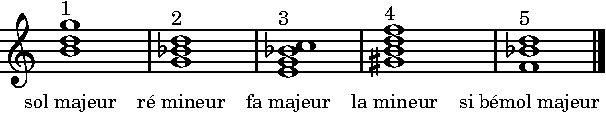
\includegraphics[scale=\echelle]{a-exercice-1.cropped.pdf}\\[10pt]
  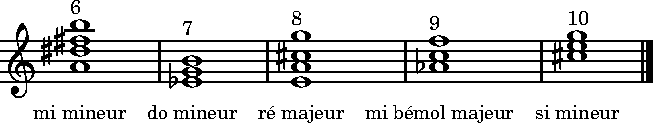
\includegraphics[scale=\echelle]{a-exercice-2.cropped.pdf}
\end{minipage}\par\medskip

\begin{remarque}
\textbf{Réponses.}
%% Produit par outils/generer_accords.py — ne pas modifier à la main.
\begin{enumerate}[leftmargin=*, itemsep=1pt]
  \item \ch{I}{6}{}~: fondamentale sol, accord parfait majeur, premier renversement.
  \item \ch{IV}{}{}~: fondamentale sol, accord parfait mineur, position fondamentale.
  \item \ch{V}{6}{5}~: fondamentale do, septième de dominante, premier renversement.
  \item \ch{VII}{7}{}~: fondamentale sol dièse, septième diminuée, position fondamentale.
  \item \ch{I}{6}{4}~: fondamentale si bémol, accord parfait majeur, deuxième renversement.
  \item \ch{V}{2}{}~: fondamentale si, septième de dominante, troisième renversement.
  \item \ch{III}{}{}~: fondamentale mi bémol, accord de quinte augmentée, position fondamentale.
  \item \ch{V}{4}{3}~: fondamentale la, septième de dominante, deuxième renversement.
  \item \ch{II}{6}{}~: fondamentale fa, accord parfait mineur, premier renversement.
  \item \ch{II}{}{}~: fondamentale do dièse, accord de quinte diminuée, position fondamentale.
\end{enumerate}

\end{remarque}

% =====================================================================
\section{Le fichier MusicXML}
\label{sec:musicxml}

Le fichier joint, \texttt{accords.musicxml}, reprend les accords de chaque
gravure, puis ceux de l'exercice, une ronde chacun à la noire 120. Il se lit
avec MuseScore, Finale, Sibelius, Dorico ou tout éditeur de partitions ; sur
slashbin.net, il s'écoute aussi dans Sodor Piano. Les chiffres et les
légendes n'y figurent pas : il sert à entendre chaque accord, et à vérifier à
l'oreille ce que disent les gravures.

% =====================================================================
\section*{Colophon}
\addcontentsline{toc}{section}{Colophon}

Les gravures musicales sont produites par \textbf{LilyPond}, la composition
par \textbf{\LaTeX}. Les accords, les tableaux, les réponses de l'exercice et
le fichier MusicXML dérivent du modèle de hauteurs des autres guides, les
modules \texttt{gammes.py} et \texttt{intervalles.py} du dossier
\texttt{outils} : un accord y est une pile de tierces prise dans une gamme.
Chaque accord construit est ensuite analysé à partir de ses seules notes,
comme le ferait un lecteur, et l'analyse doit retrouver la construction.
Avant d'écrire quoi que ce soit, le générateur vérifie sur les quinze
tonalités majeures et mineures ce que le texte affirme : la nature des
accords de chaque degré, la structure de la septième de dominante et de la
septième diminuée, le chiffrage de chaque renversement. Pour régénérer
l'ensemble :

\begin{center}
\texttt{python3 outils/generer\_accords.py}\\
\texttt{(cd gravures \&\& lilypond -dcrop --formats=pdf a-*.ly)}\\
\texttt{pdflatex accords.tex}
\end{center}

\end{document}
